%\bigskip\bigskip\bigskip % HACK
\ctitle{Genteknologi}

\paragraph{Dette kapittelet} Del 1 forklarer strukturen til organismers \ix{arvemateriale}, og hvordan kroppen bruker DNA til å lage proteiner. Del 2 forklarer hvordan man kunstig kan modifisere arvematerialet med genteknologi. Del 3 tar for seg historien til kunstig fremstilt insulin, som tar opp en del plass i boka.

\cstitle{Strukturen til DNA og RNA}

\paragraph{Byggecellene i DNA og RNA} \ix{DNA} er molekylet som inneholder den genetiske informasjonen til organismer. I eukaryote celler er DNA lagret i cellekjernen, samt i mitokondrier og kloroplaster, som har eget DNA (da disse organellene opprinnelig var bakterier med eget arvemateriale). Grunnenheten som DNA består av er en \idx{nukleotid}: en base (adenin(A), guanin(G), cytosin(C) eller tymin(T)/uracil(U) (sistnevnte er henholdsvis for DNA og RNA)) bundet til et molekyl av sukkeret \idx{deoksyribose} (eller ribose, i RNA), som så er bundet til en fosfatgruppe. 

\paragraph{Sammensetning} Nukleotidene er bundet til hverandre gjennom \ix{fosfodiesterbinding}er for å danne en polynukleotidkjede. Vi sier at kjeden har en retning, 5'$\rightarrow$3', fordi 5'-hydroksygruppen på ett nukleotid er bundet til 3'hydroksygruppen på et annet nukleotid via en fosfatgruppe. Per konvensjon begynner vi på ende-fosfatgruppen som er bundet til en 5'-hydroksygruppe.

\paragraph{Dobbeltstrengen i DNA} i DNA er hver nukleotid i en polynukleotidkjede bundet til en tilsvarende nukleotid i en annen polynukleotidkjede etter regelen \ce{A <-> T}, \ce{G <-> C}. Denne \ix{basepar}ringen skjer på grunn av hydrogenbindinger mellom basene: adenin og tymin danner to hydrogenbindinger seg imellom, guanin og cytosin danner tre hydrogenbindinger seg imellom. Dette holder DNA, som altså egentlig er to molekyler (polynukleotidkjeder), sammen som om det var ett molekyl. Derfor kommer det noe ukorrekte begrepet ``DNA-molekyl'' til å bli brukt videre i teksten.

De to strengene i DNA er antiparallelle - 3'-enden på en streng korresponderer til 5'-enden på en annen streng.

\paragraph{Replikasjon av DNA} At DNA tar form som en dobbeltstreng, gir opphav til en mekanisme for å kopiere et DNA-molekyl. De to strengene separeres, og en ny streng settes sammen ved å bruke nukleotider etter regelen for baseparing. Dermed pares hver av strengene i DNA opp med en nylig syntetisert komplementær streng, og da har man to DNA-molekyler. Enzymene som utfører denne operasjonen  heter \idx{DNA polymerase}.

\paragraph{Strukturen til RNA} RNA ligner mye på DNA, med følgende forskjeller: 
\begin{itemize}[nolistsep,noitemsep]
	\item der det er deoksyribose i DNA er det ribose i RNA
	\item der det er tymin i DNA er det uracil i RNA
	\item RNA består av én streng i stedet for to
\end{itemize}
RNA kan ha intrikate sekundærstrukturer, som gjør at det også kan danne enzymer. Ribosomer, for eksempel, er komplekser av protein og RNA.

\paragraph{Proteinsyntese} Proteiner dannes som vist i Figur \ref{fig:centraldogma}. \idx{mRNA} (messenger-RNA) syntetiseres fra DNA-et (\idx{transkripsjon}), som inneholder informasjonen som skal til for at et \ix{ribosom} kan sette sammen det riktige proteinet (\idx{translasjon}). Under translasjon er det grupper på tre baser, som kalles \ix{kodon}er, som bestemmer hvilken aminosyre som skal settes inn i polypeptidkjeden. At informasjonsflyten er DNA$\rightarrow$RNA$\rightarrow$protein, og ikke motsatt, kalles \idx{det sentrale dogmet i molekylærbiologi}. Likevel kan noen virus syntetisere DNA fra en RNA-mal gjennom reverstranskripsjon (kapittel 5).
\begin{figure}[H]
	\centering
	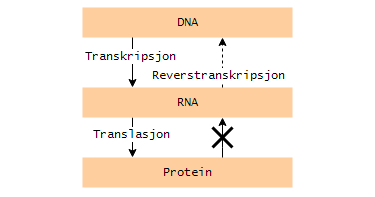
\includegraphics[width=0.45\textwidth]{centraldogma}
	\caption{Genetisk informasjonsflyt i cellen.}
	\label{fig:centraldogma}
\end{figure}
En noenlunde nøyaktig beskrivelse av veien fra DNA til protein (med korrekte molekylmodeller) finnes her: \url{https://www.youtube.com/watch?v=D3fOXt4MrOM}

\paragraph{Strukturen til et gen} Strukturelle gener \index{strukturelt gen} inneholder informasjonen som skal til for å kode enkeltproteiner, for eksempel enzymer. Ved siden av de strukturelle genene er det sekvenser som kontrollerer om genet skal uttrykkes (det vil si om det faktisk skal dannes proteiner basert på informasjonen som ligger i genet). En slik sekvens - en start-sekvens (\idx{promoter}) - en kort sekvens som enzymet RNA-polymerase kan binde seg til, før det vandrer langs DNA-kjeden og syntetiserer RNA fra og med start-sekvensen. Etter hvert møter RNA-polymerase på en stopp-sekvens (\idx{terminator}) som avslutter transkripsjonen. Mellom promoteren og det strukturelle genet finnes det ofte en \idx{operator-region} der et \idx{repressorprotein} kan sette seg fast og forhindre at genet blir uttrykt. En \idx{inducer} kan binde seg til dette proteinet på en slik måte at proteinet endrer form og forlater operator-regionen. Et eksempel på en slik inducer er sukker, som kan binde seg til repressorproteiner for gener for sukkernedbrytende enzymer. Dermed kan forskjellige gener uttrykkes avhengig av hvilke stoffer som befinner seg i organismen.

\paragraph{Rekombinasjon} Utveksling av genetisk materiale mellom to DNA-molekyler. Sammen med mutasjon er \ix{rekombinasjon} den viktigste mekanismen som fører til \ix{genetisk variasjon}. Det er mekanismen som gjør at et barn har DNA som er en blanding av DNA-et til foreldrene. Det er også en mekanisme som virus bruker for å injisere arvematerialet sitt i vertens DNA (kapittel 5).

\cstitle{Genmodifisering}

\paragraph{OBS!} Teknikkene som diskuteres i dette delkapittelet er \emph{ekstremt viktige}, og dukker opp igjen og igjen i senere kapitler. Særlig bruken av restriksjons-endonukleaser og plasmider er fundamentale verktøy.

\paragraph{Plasmider} Små ring-formede biter av DNA som finnes utenfor den mye større DNA-kjeden til bakteriene. En celle har ofte 50-100 små og 1-2 store \ix{plasmid}er, og de fleste kan reprodusere i cellen uavhengig av hoved-DNAet. De store plasmidene kan utveksles mellom bakterier i en prosess som kalles \idx{konjugering}.

\paragraph{Kloning av gener med plasmider} Konjugering kan utnyttes til å klone gener: ved å klippe opp DNA med et gen man ønsker å kopiere, samtidig som man kløyver et plasmid, og så prøver å ``smugle inn'' det ønskede genet i plasmidet med ligaser, vil det modifiserte plasmidet spre seg i bakteriekolonien slik at man etter hvert har en bakteriekoloni full av bakterier med det ønskede genet (inni et plasmid). \index{kloning av gener}

\paragraph{Restriksjons-endonukleaser} Klippingen som ble beskrevet over, gjøres med \ix{restriksjons-endonuklease}r - molekylære ``sakser''. Restriksjons-endonukleasene er hentet fra bakterier som bruker enzymet som en forsvarsmekanisme til å klippe opp virus-DNA. Det er mer enn 1200 kjente restriksjonsendonukleaser, og hver av dem er svært spesifikke (de kutter ved bestemte sekvenser på en bestemt måte). Enzymet lager et ``skjevt kutt'' slik at det er ``klebrige'' ender med enkelt-streng-DNA på hver side av kuttet. Se figur i Renneberg om akkurat hvordan dette kuttet er. Dette gjør at andre DNA-fragmenter med like ender kan hektes på (med andre enzymer som kalles \ix{DNA-ligase}r). Ved å kombinere forskjellige restriksjonsendonukleaser som danner DNA-fragmenter som passer sammen på riktig måte, kan man altså overføre gener fra ett sted til et annet.

\paragraph{Introner} For å klone et eukaryot gen kan man ikke akkurat kutte opp DNA-et, fordi det er fullt av ikke-kodende sekvenser (\ix{intron}er). I RNA danner slike introner sløyfer som kuttes av før det dannes proteiner av RNA-et, så intronene har ikke noen effekt på hvordan genet uttrykkes, men det fører til kaos når man prøver å klone genet med restriksjons-endonukleaser.

\paragraph{Kloning av eukaryote gener} Derfor trenger man heller såkalt ``voksent'' mRNA der de ovennevnte sløyfene har blitt kuttet av. Ved å bruke et enzym fra virus, revers transkriptase, kan man danne DNA fra slikt mRNA. Det resulterende kopi-DNAet (\ix{cDNA}) kan så inkorporeres i et plasmid på samme måte som beskrevet over, og proteinet man ønsker kan syntetiseres i bakterielle celler. Hvis riktig mRNA ikke er tilgjengelig er det også mulig å syntetisere akkurat de nukleotidsekvensene man vil med en \ix{DNA-synthesizer} (keyboard selges separat).

\paragraph{Hybridisering} Man har en \ix{DNA-probe} som består av en enkeltstreng med den komplementære sekvensen til den sekvensen man vet at man ønsker. Den kan for eksempel lages med en DNA-synthesizer. Proben markeres med et radioaktivt eller selvlysende molekylært ``flagg''. Proben legges til en bakteriekultur der man har ødelagt cellemembranene med vaskemiddel og spaltet dobbeltheliksen med natronlut, slik at man har en masse enkeltstrenger. Proben vil kun pare opp med sekvensen man ønsker seg, som resulterer i et hybridisert DNA av typen man ønsker seg. Så vasker man ut probene som ikke har bundet seg til noe. Hvis man har selvlysende flagg kan man enkelt identifisere en del av en bakteriekoloni som har rekombinant DNA ved å lyse på den med røntgenstråler og se på den i et mørkt rom.

\paragraph{Affinitetskromatografi}\index{affinitetskromatografi} En form for kromatografi der man utnytter at forskjellige stoffer binder seg forskjellig til spesifikke antistoffer (kapittel 5). Dette kan brukes for å foredle rekombinante proteiner man har laget fra resten av proteinene i bakterieekstraktet. For eksempel binder insulin seg mer til \ix{insulin}-antistoffer enn andre proteiner gjør. Ved å la bakterieekstraktet renne gjennom en kolonne med slike insulin-antistoffer, vil kun insulinet sette seg fast i antistoffet og forbli i kolonnen. Deretter løser man opp antistoff-insulin-bindingen med en spesifikk svak syre, slik at man ender opp med en løsning insulin er det eneste proteinet. 

\paragraph{Genmodifisering av eukaryote celler} Genmodifisering av eukaryote celler er mye mer komplisert enn det tilsvarende for prokaryote celler, fordi genmaterialet er pakket inn som kromosomer i en cellekjerne. Genet man ønsker å introdusere må injiseres inn i DNAet via en eller annen vektor (gjerne et bakterielt \ix{plasmid} med et antibiotikaresistens-gen, av grunner som blir åpenbare senere i avsnittet), men man må også sørge for at genet faktisk uttrykkes i cellen. DNA-genet man ønsker å introdusere, introduseres til plasmidet med kloningsmetodene som er beskrevet over (restriksjonsendonukleaser og ligaser). Samtidig må en startsekvens/promoter legges inn rett før genet, slik at man i sluttproduktet får et gen som faktisk blir uttrykt. Så lar man dette plasmidet forplante seg gjennom en bakteriekoloni i en løsning med et antibiotikum. Kun bakterier med det ønskelige plasmidet vil ha resistansgenet som gjør at de kan vokse og replisere på tross av antibiotikumet. Når man så har massevis av det rekombinante plasmidet, kan det introduseres i den eukaryote cellen på forskjellige måter: enten ved \ix{mikroinjeksjon} (fysisk injisere plasmidet med en veldig tynn nål, rett inn i cellekjernen, slik at plasmidet, om man er heldig, blir en del av kromosom-DNAet) eller \ix{fagocytose} (at man på et eller annet vis utnytter cellens egne mekanismer som den bruker for å ``spise opp'' partikler). Deretter gror man de eukaryote cellene i et \ix{selektivt medium} som kun lar cellene med rekombinant DNA overleve.

\cstitle{Kunstig fremstilt insulin}

\paragraph{Konvertering av griseinsulin til menneskelig \ix{insulin}} Insulin til behandling av diabetes ble i begynnelsen tatt ut fra bukspyttkjertelen til ku og gris. Slikt insulin er ikke helt likt vårt - griseinsulin er forskjellig i en av aminosyrene på enden: de har alanin der mennesker har treonin - og dette fører til bivirkninger og immunreaksjoner fordi immunsystemet kjenner igjen dyreinsulinet som forskjellig fra dens eget insulin.

En metode for å konvertere den terminale aminosyra i griseinsulin til treonin ble funnet på 80-tallet. Det viser seg at trypsin, et proteinnedbrytende enzym i magesekken, spesifikt hydrolyserer proteiner og peptider ved siden av aminosyrene lysin og arginin. I griseinsulin er alaninet man ønsker å konvertere rett ved siden av lysin, og dermed kan alaninet kløyves av insulinet ved å tilsette trypsin. Samtidig behandler man insulinet med en treonin-tertbutylester i organisk løsning, slik at treonin setter seg der alaninet var. Til slutt tilsetter man vann for å kløyve av tert-butanol, og ender opp med griseinsulin der alanin er erstattet med treonin, det vil si menneskelig insulin.

\paragraph{Rekombinant insulin fra E. coli} Insulin består av 2 separate kjeder som er bundet til hverandre med disulfidbindinger. Disse to kjedene kommer fra det samme proteinet, som har blitt spaltet i to i bukspyttkjertelen. Bakterier og gjær har ikke evnen til å gjøre dette, så direkte syntese av insulin med rekombinante plasmider er ikke mulig. For å syntetisere insulin med bakterier gror man heller to kjedene separat og setter dem sammen etterpå. På grunn av Frederick Sangers arbeid med DNA-sekvensering (kapittel 10) er basesekvensen i genet for DNA kjent, så ved å manuelt syntetisere de riktige oligonukleotidene for de to kjedene, og sette det inn i plasmid-DNA, kan man syntetisere de riktige kjedene.

Ved \ix{Asilomar-konferansen} i 1975 diskuterte noen forskere mulige risikoer ved genteknologi. For eksempel: hva om man kunne lage antibiotikaresistente karsinogene tarmbakterier og forårsake en kreft-epidemi? Eller hva om man fikk bakterier til å produsere aktivt insulin, og de ved et uhell kom seg inn i mennesker og overlevde der? Det ville forårsaket insulinsjokk. Disse hypotetiske situasjonene ble blåst opp til skremmehistorier i mediene, og National Institute of Health satt ned strenge retningslinjer for genteknologi. En konsekvens av dette var at de to kjedene i insulin måtte gros separat i forskjellige bakteriekulturer.

\paragraph{Menneskeskapte insulinvarianter} Det har blitt produsert varianter av insulin som ikke eksisterer i naturen, og som har litt andre egenskaper enn vanlig insulin. Et vanlig problem med insulin er at det når blodomløpet for sakte: høye konsentrasjoner av insulin danner heksamerer, men insulin kommer ikke inn i blodomløpet med mindre det er i form av dimerer eller monomerer. Dermed blir insulinnivået for lavt i begynnelsen, og etter hvert som insulinet brytes opp i mindre komponenter, holder nivået seg for høyt for lenge. Derfor har man produsert insulin der man har byttet plass på prolin og lysin på plass 28 og 29. Denne typen insulin fungerer raskere enn naturlig insulin. Andre varianter som fungerer enda tregere enn vanlig insulin, som varer i opp til 24 timer, forskes det også på. I slike trege varianter har man forlenget én av kjedene for å danne insulin som danner enda mindre løselige heksamerer.
